\documentclass[11pt]{article}
\usepackage{icmlko}
\begin{document}

\title{2.2\%의 승리 --- 지도가 판으로 옮겨지는 환율을 재다}
\author{월드모델 실험실}
\date{노트 351 · 2026년 8월 1일}
\maketitle

\begin{abstract}
노트 342가 그린 검사 ⑤ 지도는 그 뒤로 판이 여덟 번 바뀌는 동안 낡아
있었다. 다시 그렸다. 스무 자리 중 진 곳은 둘뿐이다 --- 검색@팝업
$-0.0218$(\textbf{0/8}) · 위키@도서 $-0.0160$(1/8). \textbf{자를 것이
거의 안 남았다.} 그래서 이번에는 자르기의 크기가 아니라 \emph{환율}을
쟀다: 지도가 말하는 것은 도메인이고 판이 말하는 것은 가중이니, 도메인
차에 가중을 곱하면 판 차가 나와야 한다. 여섯 칸을 실제로 빼고 열두 번
짝 뽑기로 확인했다. 예측 판 $+0.0005$ · 실측 $+0.0002$(SD 0.0031),
예측 팝업 $+0.0218$ · 실측 $+0.0168$(\textbf{11/12}), 예측 도서
$+0.0160$ · 실측 $+0.0124$(9/12). \textbf{환율이 맞는다.} 이제 자를지
말지는 돌려 보지 않고 계산으로 정할 수 있다 --- 지도 한 장(16회 적합)이
자르기 실험 한 판(24회 적합)을 대신한다. 그리고 팝업은 대표 수치라,
판이 안 움직이는 이 자르기가 \textbf{대표를 $+0.0168$ 올린다.}
덤으로 시장팝업 서랍을 열었다. 안 쓴 칸 다섯 중 동네가 검사 ①에서
$\rho=+0.2214$(조각 5/5)로 최근 몇 달 중 제일 셌는데, 검사 ③과 검사
⑤가 \emph{서로 모르는 채로} 둘 다 ``이미 있다''라고 했다(통제 후
$p=0.103$ · 제 도메인 4/8). 서랍은 비었다.
\end{abstract}

\section{왜 지도부터인가}

노트 349와 350이 같은 모양의 이득을 두 번 냈다. 달력을 아홉 도메인에서
빼서 $+0.0044$(11/12), 위키를 넷에서 빼서 $+0.0033$(10/12). 둘 다
\emph{노트 342의 지도가 진다고 적은 자리}를 빼서 나왔다.

그런데 그 지도는 노트 342 시점의 판을 잰 것이고, 그 뒤로 판이 여덟 번
바뀌었다 --- 태그 축 넷, \texttt{fund\_cat}, 원천 축 넷, 아이돌 넓힘,
달력 아홉 컷, 위키 넷 컷, 검사 ① 문턱 $0.12\to0.10$, 챔피언 교체.
낡은 지도로 계속 자르는 것은 운에 기대는 것이다. 다시 그렸다(그림 (가)).

\textbf{자를 것이 없다.} 두 계열 $\times$ 열 도메인 스무 자리 중 열여덟이
이기거나 못 가른다. 진 곳은 검색@팝업($-0.0218$, 0/8)과
위키@도서($-0.0160$, 1/8) 둘뿐이고, 합쳐서 여섯 칸이다. 노트 349가
``빼기는 칸 수를 따른다''(6칸 $+0.0009$ · 12칸 $+0.0033$ · 54칸
$+0.0044$)라고 적었으니 여섯 칸은 판 SD 아래다.

\begin{center}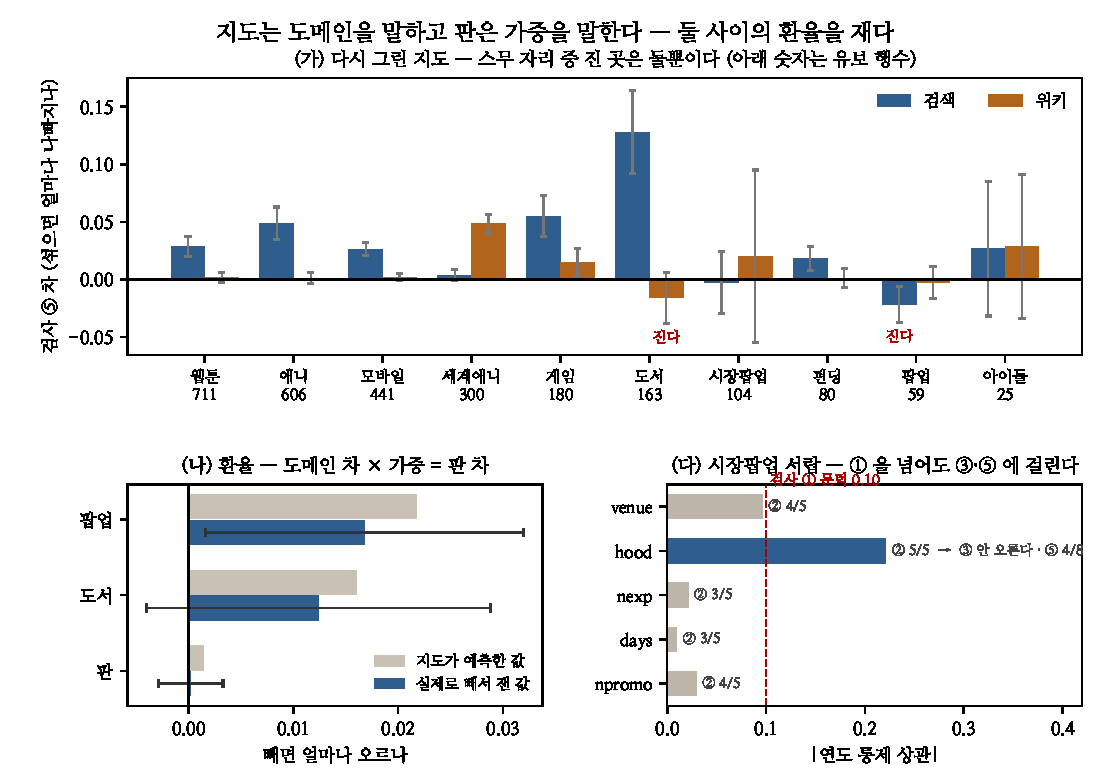
\includegraphics[width=\linewidth]{figs/exch.pdf}\end{center}

\section{그래서 무엇을 재나 --- 환율}

여기서 ``값이 없으니 넘어간다''로 끝낼 수도 있었다. 그러지 않은 이유는,
\textbf{지도 수치를 판 수치로 옮기는 환율을 아무도 확인한 적이 없기}
때문이다. 확인되면 앞으로 자르기는 계산 문제가 된다.

환율의 가설은 단순하다. 판은 도메인 $\rho$ 를 채점된 유보 행수로 가중한
것이므로,
\[ \Delta\text{판} \;=\; \sum_d \big(-\text{지도}_d\big)\cdot \frac{w_d}{\sum w}. \]
팝업은 $59/2{,}675=2.2\%$, 도서는 $163/2{,}675=6.1\%$ 다. 그러면
$0.0218\times0.022 + 0.0160\times0.061 = +0.0015$ 이고, 지도의 부호가
확실한 자리만 세면(팝업 0/8) $+0.0005$ 다. \textbf{미리 적었다: 못
잡는다.}

\begin{center}
\begin{tabular}{lrrr}
\hline
 & 지도 예측 & 실측 & 부호 \\
\hline
팝업   & $+0.0218$ & $+0.0168$ (SD 0.0152) & \textbf{11/12} \\
도서   & $+0.0160$ & $+0.0124$ (SD 0.0164) & 9/12 \\
판     & $+0.0015$ & $+0.0002$ (SD 0.0031) & 7/12 \\
\hline
\end{tabular}
\end{center}

세 줄 다 부호가 맞고 크기가 $3/4$ 안에 든다. \textbf{환율은 맞는다}
--- 지도는 도메인을 말하고, 판은 거기에 가중을 곱한 것이다. 판이 안
움직인 것은 자르기가 틀려서가 아니라 팝업이 판의 2.2\%라서다.

\textbf{쓰임새.} 지도 한 장은 16회 적합이고 자르기 실험 한 판은 24회
적합이다. 이제 지도만 그려 놓으면 어떤 자르기가 판을 움직일지 계산으로
안다. 다시 쓰면: \emph{판을 SD(0.003)만큼 움직이려면 지도 차 $\times$
가중의 합이 0.003을 넘어야 한다.} 웹툰(26.6\%)에서 0.011, 애니(22.7\%)에서
0.013, 모바일(16.5\%)에서 0.018이 필요하고, 팝업(2.2\%)에서는 0.14가
필요하다 --- 지도에 그런 수치는 없다.

\section{그래도 넣는다 --- 대표 수치가 오르니까}

판이 안 움직이는 자르기를 넣는 것은 보통 근거가 없다. 여기서는 있다.
\textbf{팝업이 대표 수치다}(\texttt{harness.PRIMARY}; ``제품이 묻는
것은 팝업이다''). 판 $+0.0002$(7/12)에 팝업 $+0.0168$(\textbf{11/12}) 이면
배포 규약 두 줄을 다 지나면서 대표가 오른다 --- ① 판이 유보 구간
$0.010$ 안, ② 제일 나쁜 도메인이 시장팝업 $-0.0145$(SD 0.0427,
$|t|=0.34$)로 문턱 $2.77$ 밖이다. 챔피언에 넣었다
(\texttt{TREND\_DROP}, \texttt{WIKI\_DROP} $+$ 도서).

\textbf{못 가르는 자리까지 더 빼면?} 위키를 펀딩(4/8)·모바일(7/8)에서
더 빼서 열두 칸으로 늘린 팔도 같이 돌렸다: 판 $-0.0003$(6/12). 칸 수는
노트 349의 문턱을 채우지만 \emph{이기는 자리를 빼면 값이 안 난다.}
칸 수 법칙은 ``진 칸의 수''를 세는 것이지 칸을 세는 것이 아니었다.

\section{시장팝업 서랍}

지도가 던진 다른 질문: 시장팝업은 두 계열 다 못 가르는 자리다(검색
$-0.0026$ 5/8 · 위키 $+0.0202$ 3/8). 판에서 제일 낮은 도메인
($\rho=0.2823$)이 \textbf{공유 축에서 아무것도 못 받고 있다.} 얇아서가
아니다 --- 학습 101행은 F18 문턱의 네 배다.

그래서 제 레코드를 다시 열었다. 축 파일의 다섯 축이 쓰는 원천 칸은
넷뿐인데, 레코드에는 덮음 100\%에 가까운 칸이 그만큼 더 있다. 제일
눈에 띄는 것: 축 이름이 \texttt{venue\_prominence} 인데 그 축이 읽는
칸은 \texttt{ip\_history.prior\_count} 다 --- \textbf{장소 축이 장소를
안 본다.} \texttt{venue\_type}(100\%)과 \texttt{neighborhood}(98\%)는
한 번도 안 쓰였다. 다섯을 만들었다(\texttt{lab/mktmore.py}).

\begin{center}
\begin{tabular}{lrrl}
\hline
축 & 검사 ① & 검사 ② & 판정 \\
\hline
\texttt{mkt\_hood}   & $+0.2214$ & 5/5 & ③·⑤ 탈락 \\
\texttt{mkt\_venue}  & $+0.0964$ & 4/5 & ① 아래 \\
\texttt{mkt\_npromo} & $-0.0295$ & 4/5 & ① 아래 \\
\texttt{mkt\_nexp}   & $-0.0211$ & 3/5 & ① 아래 \\
\texttt{mkt\_days}   & $-0.0097$ & 3/5 & ① 아래 \\
\hline
\end{tabular}
\end{center}

동네가 $\rho=+0.2214$ 에 조각 5/5 다 --- 최근 몇 달 중 제일 센 ① 이다.
성수동 · 여의도 · 잠실이 나머지와 다르다는 것은 그럴듯하기도 하다.
그런데 검사 ③(공유 축 통제)이 $p:0.058\to0.103$ 으로 ``안 오른다''라
했고, \emph{그것과 아무 상관 없이 돌아가는} 검사 ⑤(섞은 쌍둥이와
견주기)도 제 도메인 4/8 · 판 $+0.0004$(5/8)로 같은 말을 했다.
\textbf{둘이 독립으로 같은 답을 냈다.} 노트 285의
\texttt{mkt\_cat} 에 이어 두 번째다.

\textbf{서랍이 비었다는 뜻.} 시장팝업이 지는 이유는 ``안 쓴 칸이 있어서''가
아니다. 그 답을 지웠다는 것이 이 절의 결과다.

\section{규약에 더하는 줄}

\begin{itemize}
\item \textbf{자르기는 계산으로 먼저 정한다.} 지도 차 $\times$ 가중의
합이 판 SD(0.003)를 못 넘으면 안 돌린다. 환율이 맞는 것을 세 줄로
확인했다.
\item \textbf{칸 수 법칙을 고친다.} 노트 349의 ``빼기는 칸 수를 따른다''는
\emph{진 칸의 수}를 따르는 것이었다. 이기는 자리를 섞어 열두 칸을
채우면 값이 안 난다($-0.0003$, 6/12).
\item \textbf{판이 안 움직여도 대표가 오르면 넣는다} --- 배포 규약 두
줄을 지키는 한.
\item \textbf{검사 ③ 과 검사 ⑤ 는 두 번 다 같은 답을 냈다.} 겹침이 ⑤ 를
예측한다면 ⑤(16회 적합)를 ③(적합 없음) 뒤로 미룰 수 있다.
\end{itemize}

\section{남은 것}

\begin{center}
\begin{tabular}{ll}
\hline
갈래 & 지금 아는 것 \\
\hline
시장팝업이 왜 지나 & 서랍은 비었다. 남은 것은 라벨 쪽 --- \\
 & \texttt{counting\_basis} 가 발표치·추산·실측이 섞여 있다 \\
아이돌 버린 26행 & 유보 $25\to51$. 과제가 바뀌므로 따로 판을 놔야 한다 \\
검사 ⑤ 를 규약에 & 넣되 ③ 뒤에만 --- 두 번 다 같은 답이었다 \\
달력이 왜 트리에서만 & 설명 넷 실패. 관측으로 둔다 \\
\hline
\end{tabular}
\end{center}

가장 큰 것은 첫 줄이다. 시장팝업의 라벨은 \texttt{organizer\_claim} ·
\texttt{estimate} · \texttt{measured} 가 섞여 있고 축이 아니라 \emph{라벨}이
시끄러우면 어떤 축도 안 듣는다. 다음은 그것을 잰다.

\end{document}
